\documentclass[twoside]{book}

% Packages required by doxygen
\usepackage{fixltx2e}
\usepackage{calc}
\usepackage{doxygen}
\usepackage[export]{adjustbox} % also loads graphicx
\usepackage{graphicx}
\usepackage[utf8]{inputenc}
\usepackage{makeidx}
\usepackage{multicol}
\usepackage{multirow}
\PassOptionsToPackage{warn}{textcomp}
\usepackage{textcomp}
\usepackage[nointegrals]{wasysym}
\usepackage[table]{xcolor}

% Font selection
\usepackage[T1]{fontenc}
\usepackage[scaled=.90]{helvet}
\usepackage{courier}
\usepackage{amssymb}
\usepackage{sectsty}
\renewcommand{\familydefault}{\sfdefault}
\allsectionsfont{%
  \fontseries{bc}\selectfont%
  \color{darkgray}%
}
\renewcommand{\DoxyLabelFont}{%
  \fontseries{bc}\selectfont%
  \color{darkgray}%
}
\newcommand{\+}{\discretionary{\mbox{\scriptsize$\hookleftarrow$}}{}{}}

% Page & text layout
\usepackage{geometry}
\geometry{%
  a4paper,%
  top=2.5cm,%
  bottom=2.5cm,%
  left=2.5cm,%
  right=2.5cm%
}
\tolerance=750
\hfuzz=15pt
\hbadness=750
\setlength{\emergencystretch}{15pt}
\setlength{\parindent}{0cm}
\setlength{\parskip}{3ex plus 2ex minus 2ex}
\makeatletter
\renewcommand{\paragraph}{%
  \@startsection{paragraph}{4}{0ex}{-1.0ex}{1.0ex}{%
    \normalfont\normalsize\bfseries\SS@parafont%
  }%
}
\renewcommand{\subparagraph}{%
  \@startsection{subparagraph}{5}{0ex}{-1.0ex}{1.0ex}{%
    \normalfont\normalsize\bfseries\SS@subparafont%
  }%
}
\makeatother

% Headers & footers
\usepackage{fancyhdr}
\pagestyle{fancyplain}
\fancyhead[LE]{\fancyplain{}{\bfseries\thepage}}
\fancyhead[CE]{\fancyplain{}{}}
\fancyhead[RE]{\fancyplain{}{\bfseries\leftmark}}
\fancyhead[LO]{\fancyplain{}{\bfseries\rightmark}}
\fancyhead[CO]{\fancyplain{}{}}
\fancyhead[RO]{\fancyplain{}{\bfseries\thepage}}
\fancyfoot[LE]{\fancyplain{}{}}
\fancyfoot[CE]{\fancyplain{}{}}
\fancyfoot[RE]{\fancyplain{}{\bfseries\scriptsize Generated by Doxygen }}
\fancyfoot[LO]{\fancyplain{}{\bfseries\scriptsize Generated by Doxygen }}
\fancyfoot[CO]{\fancyplain{}{}}
\fancyfoot[RO]{\fancyplain{}{}}
\renewcommand{\footrulewidth}{0.4pt}
\renewcommand{\chaptermark}[1]{%
  \markboth{#1}{}%
}
\renewcommand{\sectionmark}[1]{%
  \markright{\thesection\ #1}%
}

% Indices & bibliography
\usepackage{natbib}
\usepackage[titles]{tocloft}
\setcounter{tocdepth}{3}
\setcounter{secnumdepth}{5}
\makeindex

% Hyperlinks (required, but should be loaded last)
\usepackage{ifpdf}
\ifpdf
  \usepackage[pdftex,pagebackref=true]{hyperref}
\else
  \usepackage[ps2pdf,pagebackref=true]{hyperref}
\fi
\hypersetup{%
  colorlinks=true,%
  linkcolor=blue,%
  citecolor=blue,%
  unicode%
}

% Custom commands
\newcommand{\clearemptydoublepage}{%
  \newpage{\pagestyle{empty}\cleardoublepage}%
}

\usepackage{caption}
\captionsetup{labelsep=space,justification=centering,font={bf},singlelinecheck=off,skip=4pt,position=top}

%===== C O N T E N T S =====

\begin{document}

% Titlepage & ToC
\hypersetup{pageanchor=false,
             bookmarksnumbered=true,
             pdfencoding=unicode
            }
\pagenumbering{roman}
\begin{titlepage}
\vspace*{7cm}
\begin{center}%
{\Large My Project }\\
\vspace*{1cm}
{\large Generated by Doxygen 1.8.11}\\
\end{center}
\end{titlepage}
\clearemptydoublepage
\tableofcontents
\clearemptydoublepage
\pagenumbering{arabic}
\hypersetup{pageanchor=true}

%--- Begin generated contents ---
\chapter{Class Index}
\section{Class List}
Here are the classes, structs, unions and interfaces with brief descriptions\+:\begin{DoxyCompactList}
\item\contentsline{section}{\hyperlink{classedge}{edge} }{\pageref{classedge}}{}
\item\contentsline{section}{\hyperlink{classmodel__2d}{model\+\_\+2d} }{\pageref{classmodel__2d}}{}
\item\contentsline{section}{\hyperlink{classmodel__3d}{model\+\_\+3d} }{\pageref{classmodel__3d}}{}
\item\contentsline{section}{\hyperlink{classsurface}{surface} }{\pageref{classsurface}}{}
\item\contentsline{section}{\hyperlink{classvertex}{vertex} }{\pageref{classvertex}}{}
\end{DoxyCompactList}

\chapter{Class Documentation}
\hypertarget{classedge}{}\section{edge Class Reference}
\label{classedge}\index{edge@{edge}}


Collaboration diagram for edge\+:
\nopagebreak
\begin{figure}[H]
\begin{center}
\leavevmode
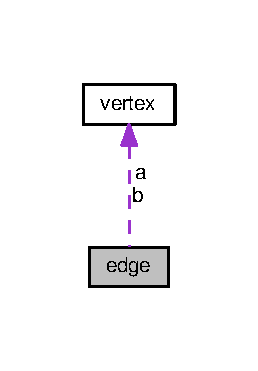
\includegraphics[width=124pt]{classedge__coll__graph}
\end{center}
\end{figure}
\subsection*{Public Member Functions}
\begin{DoxyCompactItemize}
\item 
\hyperlink{classedge_ac8047a0d7c1e08a4063be409c6fd0a88}{edge} ()
\item 
\hyperlink{classedge_ac18a14c98d747852a75b022fc8bb2588}{edge} (\hyperlink{classvertex}{vertex} $\ast$a, \hyperlink{classvertex}{vertex} $\ast$b, int c)
\item 
\hyperlink{classvertex}{vertex} $\ast$ \hyperlink{classedge_a94884123402ed9847db2262603946728}{get\+\_\+neighbour} (\hyperlink{classvertex}{vertex} $\ast$d)
\item 
\hyperlink{classvertex}{vertex} $\ast$ \hyperlink{classedge_a5624f749846113812f2e7b58e60d0b05}{midpoint} ()
\item 
\hyperlink{classedge}{edge} $\ast$ \hyperlink{classedge_aec9e483e97c42b20838ff0b787026801}{get\+\_\+edge} ()
\end{DoxyCompactItemize}
\subsection*{Public Attributes}
\begin{DoxyCompactItemize}
\item 
\hyperlink{classvertex}{vertex} $\ast$ {\bfseries a}\hypertarget{classedge_a495730f8eb651105b809ea702622c6e6}{}\label{classedge_a495730f8eb651105b809ea702622c6e6}

\item 
\hyperlink{classvertex}{vertex} $\ast$ {\bfseries b}\hypertarget{classedge_a14e5fc116c7aa31f149f579c9c9883fc}{}\label{classedge_a14e5fc116c7aa31f149f579c9c9883fc}

\item 
bool {\bfseries hidden}\hypertarget{classedge_a58e9f0be7697205f09966afeb70bd459}{}\label{classedge_a58e9f0be7697205f09966afeb70bd459}

\item 
bool {\bfseries istrue}\hypertarget{classedge_ab10731d146d60f95cb22c684a47bd737}{}\label{classedge_ab10731d146d60f95cb22c684a47bd737}

\item 
int {\bfseries eno}\hypertarget{classedge_adea185395d6e606e36a0bd0236e64044}{}\label{classedge_adea185395d6e606e36a0bd0236e64044}

\end{DoxyCompactItemize}


\subsection{Constructor \& Destructor Documentation}
\index{edge@{edge}!edge@{edge}}
\index{edge@{edge}!edge@{edge}}
\subsubsection[{\texorpdfstring{edge()}{edge()}}]{\setlength{\rightskip}{0pt plus 5cm}edge\+::edge (
\begin{DoxyParamCaption}
{}
\end{DoxyParamCaption}
)}\hypertarget{classedge_ac8047a0d7c1e08a4063be409c6fd0a88}{}\label{classedge_ac8047a0d7c1e08a4063be409c6fd0a88}
Default Constructor\index{edge@{edge}!edge@{edge}}
\index{edge@{edge}!edge@{edge}}
\subsubsection[{\texorpdfstring{edge(vertex $\ast$a, vertex $\ast$b, int c)}{edge(vertex *a, vertex *b, int c)}}]{\setlength{\rightskip}{0pt plus 5cm}edge\+::edge (
\begin{DoxyParamCaption}
\item[{{\bf vertex} $\ast$}]{a, }
\item[{{\bf vertex} $\ast$}]{b, }
\item[{int}]{c}
\end{DoxyParamCaption}
)}\hypertarget{classedge_ac18a14c98d747852a75b022fc8bb2588}{}\label{classedge_ac18a14c98d747852a75b022fc8bb2588}
Set Edge with pointers to vertices

\subsection{Member Function Documentation}
\index{edge@{edge}!get\+\_\+edge@{get\+\_\+edge}}
\index{get\+\_\+edge@{get\+\_\+edge}!edge@{edge}}
\subsubsection[{\texorpdfstring{get\+\_\+edge()}{get_edge()}}]{\setlength{\rightskip}{0pt plus 5cm}{\bf edge} $\ast$ edge\+::get\+\_\+edge (
\begin{DoxyParamCaption}
{}
\end{DoxyParamCaption}
)}\hypertarget{classedge_aec9e483e97c42b20838ff0b787026801}{}\label{classedge_aec9e483e97c42b20838ff0b787026801}
Return the edge object\index{edge@{edge}!get\+\_\+neighbour@{get\+\_\+neighbour}}
\index{get\+\_\+neighbour@{get\+\_\+neighbour}!edge@{edge}}
\subsubsection[{\texorpdfstring{get\+\_\+neighbour(vertex $\ast$d)}{get_neighbour(vertex *d)}}]{\setlength{\rightskip}{0pt plus 5cm}{\bf vertex} $\ast$ edge\+::get\+\_\+neighbour (
\begin{DoxyParamCaption}
\item[{{\bf vertex} $\ast$}]{d}
\end{DoxyParamCaption}
)}\hypertarget{classedge_a94884123402ed9847db2262603946728}{}\label{classedge_a94884123402ed9847db2262603946728}
Add a surface to list of adjacent surfaces Get the neighboring vertex of a vertex with corresponding edge\index{edge@{edge}!midpoint@{midpoint}}
\index{midpoint@{midpoint}!edge@{edge}}
\subsubsection[{\texorpdfstring{midpoint()}{midpoint()}}]{\setlength{\rightskip}{0pt plus 5cm}{\bf vertex} $\ast$ edge\+::midpoint (
\begin{DoxyParamCaption}
{}
\end{DoxyParamCaption}
)}\hypertarget{classedge_a5624f749846113812f2e7b58e60d0b05}{}\label{classedge_a5624f749846113812f2e7b58e60d0b05}
Return the vertex corresponding to mid point of the edge

The documentation for this class was generated from the following files\+:\begin{DoxyCompactItemize}
\item 
edge.\+h\item 
edge.\+cpp\end{DoxyCompactItemize}

\hypertarget{classmodel__2d}{}\section{model\+\_\+2d Class Reference}
\label{classmodel__2d}\index{model\+\_\+2d@{model\+\_\+2d}}
\subsection*{Public Member Functions}
\begin{DoxyCompactItemize}
\item 
\hyperlink{classvertex}{vertex} $\ast$ \hyperlink{classmodel__2d_a7251a94523aa05a09203afd174b59ce1}{is\+\_\+intersect} (int a, int b)
\item 
void {\bfseries do\+\_\+intersect} (\hyperlink{classedge}{edge} $\ast$a, \hyperlink{classedge}{edge} $\ast$b)\hypertarget{classmodel__2d_a910a02de5a425bf7246fa578f5c23538}{}\label{classmodel__2d_a910a02de5a425bf7246fa578f5c23538}

\item 
void \hyperlink{classmodel__2d_a742ce3e9f537045a3e4fbf9aa1446c35}{add\+\_\+vertices} (vector$<$ \hyperlink{classvertex}{vertex} $\ast$ $>$ vt)
\item 
void \hyperlink{classmodel__2d_a61f0e93c47c4f4cec43d75b39a586db2}{add\+\_\+edges} (vector$<$ \hyperlink{classedge}{edge} $\ast$ $>$ et)
\item 
void \hyperlink{classmodel__2d_a0b1a57e36ba970523f063c61b77a7fdf}{add\+\_\+vertex} (\hyperlink{classvertex}{vertex} $\ast$vt)
\item 
vector$<$ \hyperlink{classvertex}{vertex} $\ast$ $>$ \hyperlink{classmodel__2d_a8d280c7ae53f602fff085fef1c57f81b}{ret\+\_\+vertices} ()
\item 
vector$<$ \hyperlink{classedge}{edge} $\ast$ $>$ \hyperlink{classmodel__2d_aafdd2f5684e7550dd5fb18b8543a16d9}{ret\+\_\+edges} ()
\item 
\hyperlink{classmodel__2d}{model\+\_\+2d} $\ast$ {\bfseries return\+\_\+model} ()\hypertarget{classmodel__2d_a635b8a014da2989cbec94c7acd38d0e4}{}\label{classmodel__2d_a635b8a014da2989cbec94c7acd38d0e4}

\item 
void \hyperlink{classmodel__2d_a03c3b12aaca8688832f4bc7d5301b5fe}{display\+\_\+model} ()
\item 
bool \hyperlink{classmodel__2d_a9615c9abb5627d8742ccddf03cbeae91}{on\+Segment} (pair$<$ float, float $>$ p, pair$<$ float, float $>$ q, pair$<$ float, float $>$ r)
\item 
int \hyperlink{classmodel__2d_a5d04aa594874b332d9938df13bff0d54}{orientation} (pair$<$ float, float $>$ p, pair$<$ float, float $>$ q, pair$<$ float, float $>$ r)
\item 
bool \hyperlink{classmodel__2d_ad61a6338b0631bbe61ab6caeab36ebaf}{do\+Intersect} (pair$<$ float, float $>$ p1, pair$<$ float, float $>$ q1, pair$<$ float, float $>$ p2, pair$<$ float, float $>$ q2)
\item 
bool \hyperlink{classmodel__2d_ab09798577266c0d7a83de6bbeb3a5f32}{isinside} (\hyperlink{classvertex}{vertex} $\ast$t, int q)
\item 
void \hyperlink{classmodel__2d_a1244480a2e46cf85f622324895855e98}{dispvertex} ()
\item 
void \hyperlink{classmodel__2d_a41dbf981ec2c7df95bd227aded96e99a}{dispedge} ()
\item 
void \hyperlink{classmodel__2d_a4a1ba007053ebe9bd443abaeeda8df83}{dispsurface} ()
\end{DoxyCompactItemize}
\subsection*{Public Attributes}
\begin{DoxyCompactItemize}
\item 
int {\bfseries direction}\hypertarget{classmodel__2d_a549e12acad9d94f8115252497524cf19}{}\label{classmodel__2d_a549e12acad9d94f8115252497524cf19}

\item 
vector$<$ \hyperlink{classvertex}{vertex} $\ast$ $>$ {\bfseries v}\hypertarget{classmodel__2d_acb0399caf2660e0203e473969fbe9d27}{}\label{classmodel__2d_acb0399caf2660e0203e473969fbe9d27}

\item 
vector$<$ \hyperlink{classedge}{edge} $\ast$ $>$ {\bfseries e}\hypertarget{classmodel__2d_a3b4836d70d42e5c2ed90a8495c430a0f}{}\label{classmodel__2d_a3b4836d70d42e5c2ed90a8495c430a0f}

\item 
vector$<$ \hyperlink{classsurface}{surface} $\ast$ $>$ {\bfseries s}\hypertarget{classmodel__2d_aa4aaa097b9f187e9806981ad33368f35}{}\label{classmodel__2d_aa4aaa097b9f187e9806981ad33368f35}

\end{DoxyCompactItemize}


\subsection{Member Function Documentation}
\index{model\+\_\+2d@{model\+\_\+2d}!add\+\_\+edges@{add\+\_\+edges}}
\index{add\+\_\+edges@{add\+\_\+edges}!model\+\_\+2d@{model\+\_\+2d}}
\subsubsection[{\texorpdfstring{add\+\_\+edges(vector$<$ edge $\ast$ $>$ et)}{add_edges(vector< edge * > et)}}]{\setlength{\rightskip}{0pt plus 5cm}void model\+\_\+2d\+::add\+\_\+edges (
\begin{DoxyParamCaption}
\item[{vector$<$ {\bf edge} $\ast$ $>$}]{et}
\end{DoxyParamCaption}
)}\hypertarget{classmodel__2d_a61f0e93c47c4f4cec43d75b39a586db2}{}\label{classmodel__2d_a61f0e93c47c4f4cec43d75b39a586db2}
Adding edges to this 2d model\index{model\+\_\+2d@{model\+\_\+2d}!add\+\_\+vertex@{add\+\_\+vertex}}
\index{add\+\_\+vertex@{add\+\_\+vertex}!model\+\_\+2d@{model\+\_\+2d}}
\subsubsection[{\texorpdfstring{add\+\_\+vertex(vertex $\ast$vt)}{add_vertex(vertex *vt)}}]{\setlength{\rightskip}{0pt plus 5cm}void model\+\_\+2d\+::add\+\_\+vertex (
\begin{DoxyParamCaption}
\item[{{\bf vertex} $\ast$}]{vt}
\end{DoxyParamCaption}
)}\hypertarget{classmodel__2d_a0b1a57e36ba970523f063c61b77a7fdf}{}\label{classmodel__2d_a0b1a57e36ba970523f063c61b77a7fdf}
Add a single vertex to this 2d model\index{model\+\_\+2d@{model\+\_\+2d}!add\+\_\+vertices@{add\+\_\+vertices}}
\index{add\+\_\+vertices@{add\+\_\+vertices}!model\+\_\+2d@{model\+\_\+2d}}
\subsubsection[{\texorpdfstring{add\+\_\+vertices(vector$<$ vertex $\ast$ $>$ vt)}{add_vertices(vector< vertex * > vt)}}]{\setlength{\rightskip}{0pt plus 5cm}void model\+\_\+2d\+::add\+\_\+vertices (
\begin{DoxyParamCaption}
\item[{vector$<$ {\bf vertex} $\ast$ $>$}]{vt}
\end{DoxyParamCaption}
)}\hypertarget{classmodel__2d_a742ce3e9f537045a3e4fbf9aa1446c35}{}\label{classmodel__2d_a742ce3e9f537045a3e4fbf9aa1446c35}
Adding vertices to this 2d model\index{model\+\_\+2d@{model\+\_\+2d}!dispedge@{dispedge}}
\index{dispedge@{dispedge}!model\+\_\+2d@{model\+\_\+2d}}
\subsubsection[{\texorpdfstring{dispedge()}{dispedge()}}]{\setlength{\rightskip}{0pt plus 5cm}void model\+\_\+2d\+::dispedge (
\begin{DoxyParamCaption}
{}
\end{DoxyParamCaption}
)}\hypertarget{classmodel__2d_a41dbf981ec2c7df95bd227aded96e99a}{}\label{classmodel__2d_a41dbf981ec2c7df95bd227aded96e99a}
Display the lsit of edges of the polygon\index{model\+\_\+2d@{model\+\_\+2d}!display\+\_\+model@{display\+\_\+model}}
\index{display\+\_\+model@{display\+\_\+model}!model\+\_\+2d@{model\+\_\+2d}}
\subsubsection[{\texorpdfstring{display\+\_\+model()}{display_model()}}]{\setlength{\rightskip}{0pt plus 5cm}void model\+\_\+2d\+::display\+\_\+model (
\begin{DoxyParamCaption}
{}
\end{DoxyParamCaption}
)}\hypertarget{classmodel__2d_a03c3b12aaca8688832f4bc7d5301b5fe}{}\label{classmodel__2d_a03c3b12aaca8688832f4bc7d5301b5fe}
-\/\+Display the 3d solid model formed in the end.~\newline
-\/\+Uses the graphic library to display the 3d solid model.~\newline


Display the complete 2D model in the form of vertices, edges and surfaces\index{model\+\_\+2d@{model\+\_\+2d}!dispsurface@{dispsurface}}
\index{dispsurface@{dispsurface}!model\+\_\+2d@{model\+\_\+2d}}
\subsubsection[{\texorpdfstring{dispsurface()}{dispsurface()}}]{\setlength{\rightskip}{0pt plus 5cm}void model\+\_\+2d\+::dispsurface (
\begin{DoxyParamCaption}
{}
\end{DoxyParamCaption}
)}\hypertarget{classmodel__2d_a4a1ba007053ebe9bd443abaeeda8df83}{}\label{classmodel__2d_a4a1ba007053ebe9bd443abaeeda8df83}
Display the list of surfaces giving all the necessary details of the edges\index{model\+\_\+2d@{model\+\_\+2d}!dispvertex@{dispvertex}}
\index{dispvertex@{dispvertex}!model\+\_\+2d@{model\+\_\+2d}}
\subsubsection[{\texorpdfstring{dispvertex()}{dispvertex()}}]{\setlength{\rightskip}{0pt plus 5cm}void model\+\_\+2d\+::dispvertex (
\begin{DoxyParamCaption}
{}
\end{DoxyParamCaption}
)}\hypertarget{classmodel__2d_a1244480a2e46cf85f622324895855e98}{}\label{classmodel__2d_a1244480a2e46cf85f622324895855e98}
Display the list of vertices\index{model\+\_\+2d@{model\+\_\+2d}!do\+Intersect@{do\+Intersect}}
\index{do\+Intersect@{do\+Intersect}!model\+\_\+2d@{model\+\_\+2d}}
\subsubsection[{\texorpdfstring{do\+Intersect(pair$<$ float, float $>$ p1, pair$<$ float, float $>$ q1, pair$<$ float, float $>$ p2, pair$<$ float, float $>$ q2)}{doIntersect(pair< float, float > p1, pair< float, float > q1, pair< float, float > p2, pair< float, float > q2)}}]{\setlength{\rightskip}{0pt plus 5cm}bool model\+\_\+2d\+::do\+Intersect (
\begin{DoxyParamCaption}
\item[{pair$<$ float, float $>$}]{p1, }
\item[{pair$<$ float, float $>$}]{q1, }
\item[{pair$<$ float, float $>$}]{p2, }
\item[{pair$<$ float, float $>$}]{q2}
\end{DoxyParamCaption}
)}\hypertarget{classmodel__2d_ad61a6338b0631bbe61ab6caeab36ebaf}{}\label{classmodel__2d_ad61a6338b0631bbe61ab6caeab36ebaf}
Returns true if two line segments P1\+Q1 and P2\+Q2 intersect.\index{model\+\_\+2d@{model\+\_\+2d}!is\+\_\+intersect@{is\+\_\+intersect}}
\index{is\+\_\+intersect@{is\+\_\+intersect}!model\+\_\+2d@{model\+\_\+2d}}
\subsubsection[{\texorpdfstring{is\+\_\+intersect(int a, int b)}{is_intersect(int a, int b)}}]{\setlength{\rightskip}{0pt plus 5cm}{\bf vertex} $\ast$ model\+\_\+2d\+::is\+\_\+intersect (
\begin{DoxyParamCaption}
\item[{int}]{a, }
\item[{int}]{b}
\end{DoxyParamCaption}
)}\hypertarget{classmodel__2d_a7251a94523aa05a09203afd174b59ce1}{}\label{classmodel__2d_a7251a94523aa05a09203afd174b59ce1}
Checks whether the two edges intersect or not and if they do, adds the intersection vertex to list of vertices and updates the list of edges with new edges replacing the old ones too.\index{model\+\_\+2d@{model\+\_\+2d}!isinside@{isinside}}
\index{isinside@{isinside}!model\+\_\+2d@{model\+\_\+2d}}
\subsubsection[{\texorpdfstring{isinside(vertex $\ast$t, int q)}{isinside(vertex *t, int q)}}]{\setlength{\rightskip}{0pt plus 5cm}bool model\+\_\+2d\+::isinside (
\begin{DoxyParamCaption}
\item[{{\bf vertex} $\ast$}]{t, }
\item[{int}]{q}
\end{DoxyParamCaption}
)}\hypertarget{classmodel__2d_ab09798577266c0d7a83de6bbeb3a5f32}{}\label{classmodel__2d_ab09798577266c0d7a83de6bbeb3a5f32}
Point in a polygon algorithm! Checks whether a given point is inside or outside the surface\index{model\+\_\+2d@{model\+\_\+2d}!on\+Segment@{on\+Segment}}
\index{on\+Segment@{on\+Segment}!model\+\_\+2d@{model\+\_\+2d}}
\subsubsection[{\texorpdfstring{on\+Segment(pair$<$ float, float $>$ p, pair$<$ float, float $>$ q, pair$<$ float, float $>$ r)}{onSegment(pair< float, float > p, pair< float, float > q, pair< float, float > r)}}]{\setlength{\rightskip}{0pt plus 5cm}bool model\+\_\+2d\+::on\+Segment (
\begin{DoxyParamCaption}
\item[{pair$<$ float, float $>$}]{p, }
\item[{pair$<$ float, float $>$}]{q, }
\item[{pair$<$ float, float $>$}]{r}
\end{DoxyParamCaption}
)}\hypertarget{classmodel__2d_a9615c9abb5627d8742ccddf03cbeae91}{}\label{classmodel__2d_a9615c9abb5627d8742ccddf03cbeae91}
Returns whether Q lies on line segment PR or not, given P, Q and R are collinear.\index{model\+\_\+2d@{model\+\_\+2d}!orientation@{orientation}}
\index{orientation@{orientation}!model\+\_\+2d@{model\+\_\+2d}}
\subsubsection[{\texorpdfstring{orientation(pair$<$ float, float $>$ p, pair$<$ float, float $>$ q, pair$<$ float, float $>$ r)}{orientation(pair< float, float > p, pair< float, float > q, pair< float, float > r)}}]{\setlength{\rightskip}{0pt plus 5cm}int model\+\_\+2d\+::orientation (
\begin{DoxyParamCaption}
\item[{pair$<$ float, float $>$}]{p, }
\item[{pair$<$ float, float $>$}]{q, }
\item[{pair$<$ float, float $>$}]{r}
\end{DoxyParamCaption}
)}\hypertarget{classmodel__2d_a5d04aa594874b332d9938df13bff0d54}{}\label{classmodel__2d_a5d04aa594874b332d9938df13bff0d54}
Returns the orientation of point Q with respect to line segment PR Returns 0 if they are collinear, 1 if clockwise, and 3 if anti clockwise.\index{model\+\_\+2d@{model\+\_\+2d}!ret\+\_\+edges@{ret\+\_\+edges}}
\index{ret\+\_\+edges@{ret\+\_\+edges}!model\+\_\+2d@{model\+\_\+2d}}
\subsubsection[{\texorpdfstring{ret\+\_\+edges()}{ret_edges()}}]{\setlength{\rightskip}{0pt plus 5cm}vector$<$ {\bf edge} $\ast$ $>$ model\+\_\+2d\+::ret\+\_\+edges (
\begin{DoxyParamCaption}
{}
\end{DoxyParamCaption}
)}\hypertarget{classmodel__2d_aafdd2f5684e7550dd5fb18b8543a16d9}{}\label{classmodel__2d_aafdd2f5684e7550dd5fb18b8543a16d9}
cout$<$$<$\char`\"{}1 \char`\"{}$<$$<$p$<$$<$\char`\"{} \char`\"{}$<$$<$q$<$$<$endl; Returns the list of edges\index{model\+\_\+2d@{model\+\_\+2d}!ret\+\_\+vertices@{ret\+\_\+vertices}}
\index{ret\+\_\+vertices@{ret\+\_\+vertices}!model\+\_\+2d@{model\+\_\+2d}}
\subsubsection[{\texorpdfstring{ret\+\_\+vertices()}{ret_vertices()}}]{\setlength{\rightskip}{0pt plus 5cm}vector$<$ {\bf vertex} $\ast$ $>$ model\+\_\+2d\+::ret\+\_\+vertices (
\begin{DoxyParamCaption}
{}
\end{DoxyParamCaption}
)}\hypertarget{classmodel__2d_a8d280c7ae53f602fff085fef1c57f81b}{}\label{classmodel__2d_a8d280c7ae53f602fff085fef1c57f81b}
Returns the list of vertices

The documentation for this class was generated from the following files\+:\begin{DoxyCompactItemize}
\item 
model\+\_\+2d.\+h\item 
model\+\_\+2d.\+cpp\end{DoxyCompactItemize}

\hypertarget{classmodel__3d}{}\section{model\+\_\+3d Class Reference}
\label{classmodel__3d}\index{model\+\_\+3d@{model\+\_\+3d}}


Collaboration diagram for model\+\_\+3d\+:
\nopagebreak
\begin{figure}[H]
\begin{center}
\leavevmode
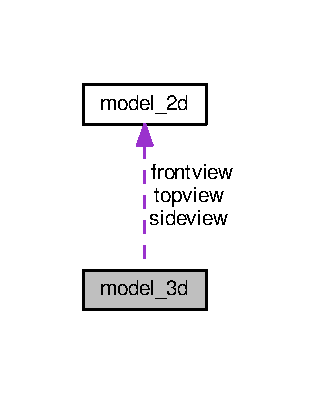
\includegraphics[width=153pt]{classmodel__3d__coll__graph}
\end{center}
\end{figure}
\subsection*{Public Member Functions}
\begin{DoxyCompactItemize}
\item 
void \hyperlink{classmodel__3d_a34719029f1c5a2bc5a609dffc741a2e4}{calc\+\_\+2d} (int direction)
\item 
\hyperlink{classmodel__2d}{model\+\_\+2d} $\ast$ \hyperlink{classmodel__3d_aa08ac7e10a9531d7b7f8fb70b65cce82}{basic\+\_\+proj} (int)
\item 
void \hyperlink{classmodel__3d_acb0cca59029c43fe4b87b5e1b3df48f0}{calc\+\_\+2d\+\_\+1} (int)
\item 
void \hyperlink{classmodel__3d_abc9c2cf8a0cd04a2a4cf1ce910672e76}{form\+\_\+wireframe} ()
\item 
void \hyperlink{classmodel__3d_a4e8d422205e9cbdd9048942a886700f3}{form\+\_\+3dfaces} ()
\item 
vector$<$ int $>$ \hyperlink{classmodel__3d_aabe53d192ed2dcd0157f61d24281dae2}{get\+\_\+neighbours} (\hyperlink{classvertex}{vertex} $\ast$vn)
\item 
\hyperlink{classedge}{edge} $\ast$ \hyperlink{classmodel__3d_ac834293db65510af4bd5baf0868f7bf3}{is\+\_\+edge} (int a, int b)
\item 
void \hyperlink{classmodel__3d_aadab2be6e920f20d58199e77c0e1a52b}{model\+\_\+3d\+\_\+verification} ()
\item 
void {\bfseries add\+\_\+vertex} (float x, float y, float z)\hypertarget{classmodel__3d_a8cdabecc29969b9b33d36c28af97835a}{}\label{classmodel__3d_a8cdabecc29969b9b33d36c28af97835a}

\item 
void {\bfseries add\+\_\+edge} (\hyperlink{classvertex}{vertex} $\ast$a, \hyperlink{classvertex}{vertex} $\ast$b)\hypertarget{classmodel__3d_a33e7bbfd961d698348e90469fb31d0aa}{}\label{classmodel__3d_a33e7bbfd961d698348e90469fb31d0aa}

\item 
void {\bfseries add\+\_\+surface} (vector$<$ \hyperlink{classedge}{edge} $\ast$ $>$ edges)\hypertarget{classmodel__3d_abf25bf8046997fdb9f39cfdedeea5d4b}{}\label{classmodel__3d_abf25bf8046997fdb9f39cfdedeea5d4b}

\item 
\hyperlink{classmodel__2d}{model\+\_\+2d} {\bfseries get\+\_\+2dview} (int direction)\hypertarget{classmodel__3d_a5a1b03401cf803eca587981650ec7bce}{}\label{classmodel__3d_a5a1b03401cf803eca587981650ec7bce}

\item 
void {\bfseries input\+\_\+2dview} (vector$<$ \hyperlink{classvertex}{vertex} $\ast$ $>$ v1, vector$<$ \hyperlink{classedge}{edge} $\ast$ $>$ e1, int direction)\hypertarget{classmodel__3d_af86b714c5ac6732e4127400283a00155}{}\label{classmodel__3d_af86b714c5ac6732e4127400283a00155}

\item 
void \hyperlink{classmodel__3d_a759ba04f608f0f49622e67d158b54d26}{display\+\_\+wireframe} ()
\item 
void \hyperlink{classmodel__3d_a2814763ae3e114fbd8f73b9f59a93c46}{display\+\_\+3d\+\_\+model} ()
\item 
void {\bfseries generate\+\_\+3d} ()\hypertarget{classmodel__3d_a8c66ba2bd9a3c58f1245db43d2b9f80f}{}\label{classmodel__3d_a8c66ba2bd9a3c58f1245db43d2b9f80f}

\item 
void \hyperlink{classmodel__3d_aec3a3507db23d9760aad5a185055767b}{dispvertex} ()
\item 
void \hyperlink{classmodel__3d_a96c90da2bbd278d2216e9ec2ce3202ed}{dispedge} ()
\item 
void \hyperlink{classmodel__3d_aff96d90d947d43be43e360a00d7f58d9}{dispsurface} ()
\item 
void \hyperlink{classmodel__3d_a1fd25e51ac11352b59029881144a0cee}{save2\+Dmodels} (fstream \&out)
\item 
void \hyperlink{classmodel__3d_a81258ba879d85e5a286cecb3e85356a2}{save3\+Dmodel} (fstream \&out)
\end{DoxyCompactItemize}
\subsection*{Public Attributes}
\begin{DoxyCompactItemize}
\item 
vector$<$ \hyperlink{classvertex}{vertex} $\ast$ $>$ {\bfseries v}\hypertarget{classmodel__3d_a885447b3fe8eb36ef06c2acfed081748}{}\label{classmodel__3d_a885447b3fe8eb36ef06c2acfed081748}

\item 
vector$<$ \hyperlink{classedge}{edge} $\ast$ $>$ {\bfseries e}\hypertarget{classmodel__3d_ab14b5fa5e0c24619f350fcc74c250dfb}{}\label{classmodel__3d_ab14b5fa5e0c24619f350fcc74c250dfb}

\item 
vector$<$ \hyperlink{classsurface}{surface} $\ast$ $>$ {\bfseries s}\hypertarget{classmodel__3d_ad4fb11609a96c41efc97af28e7c21d09}{}\label{classmodel__3d_ad4fb11609a96c41efc97af28e7c21d09}

\item 
\hyperlink{classmodel__2d}{model\+\_\+2d} $\ast$ {\bfseries topview}\hypertarget{classmodel__3d_abe594e82f1e50735959a67d38cebeff4}{}\label{classmodel__3d_abe594e82f1e50735959a67d38cebeff4}

\item 
\hyperlink{classmodel__2d}{model\+\_\+2d} $\ast$ {\bfseries frontview}\hypertarget{classmodel__3d_a83eac02f0137aa2508f65a5a2ad5cc05}{}\label{classmodel__3d_a83eac02f0137aa2508f65a5a2ad5cc05}

\item 
\hyperlink{classmodel__2d}{model\+\_\+2d} $\ast$ {\bfseries sideview}\hypertarget{classmodel__3d_afc33bd4eb2f547742e6afb481808c5db}{}\label{classmodel__3d_afc33bd4eb2f547742e6afb481808c5db}

\end{DoxyCompactItemize}


\subsection{Member Function Documentation}
\index{model\+\_\+3d@{model\+\_\+3d}!basic\+\_\+proj@{basic\+\_\+proj}}
\index{basic\+\_\+proj@{basic\+\_\+proj}!model\+\_\+3d@{model\+\_\+3d}}
\subsubsection[{\texorpdfstring{basic\+\_\+proj(int)}{basic_proj(int)}}]{\setlength{\rightskip}{0pt plus 5cm}{\bf model\+\_\+2d} $\ast$ model\+\_\+3d\+::basic\+\_\+proj (
\begin{DoxyParamCaption}
\item[{int}]{direction}
\end{DoxyParamCaption}
)}\hypertarget{classmodel__3d_aa08ac7e10a9531d7b7f8fb70b65cce82}{}\label{classmodel__3d_aa08ac7e10a9531d7b7f8fb70b65cce82}
Develop a basic 2D projection of the given 3D solid without ay hidden lines. Just the 2D projections\index{model\+\_\+3d@{model\+\_\+3d}!calc\+\_\+2d@{calc\+\_\+2d}}
\index{calc\+\_\+2d@{calc\+\_\+2d}!model\+\_\+3d@{model\+\_\+3d}}
\subsubsection[{\texorpdfstring{calc\+\_\+2d(int direction)}{calc_2d(int direction)}}]{\setlength{\rightskip}{0pt plus 5cm}void model\+\_\+3d\+::calc\+\_\+2d (
\begin{DoxyParamCaption}
\item[{int}]{direction}
\end{DoxyParamCaption}
)}\hypertarget{classmodel__3d_a34719029f1c5a2bc5a609dffc741a2e4}{}\label{classmodel__3d_a34719029f1c5a2bc5a609dffc741a2e4}
Performs segmentation of edges in 2D views i.\+e. if two edges of a 3D model intersect in 2D view, then the 2D edges are segmented so that the segmented part can be individually tested for hidden nature.\index{model\+\_\+3d@{model\+\_\+3d}!calc\+\_\+2d\+\_\+1@{calc\+\_\+2d\+\_\+1}}
\index{calc\+\_\+2d\+\_\+1@{calc\+\_\+2d\+\_\+1}!model\+\_\+3d@{model\+\_\+3d}}
\subsubsection[{\texorpdfstring{calc\+\_\+2d\+\_\+1(int)}{calc_2d_1(int)}}]{\setlength{\rightskip}{0pt plus 5cm}void model\+\_\+3d\+::calc\+\_\+2d\+\_\+1 (
\begin{DoxyParamCaption}
\item[{int}]{direction}
\end{DoxyParamCaption}
)}\hypertarget{classmodel__3d_acb0cca59029c43fe4b87b5e1b3df48f0}{}\label{classmodel__3d_acb0cca59029c43fe4b87b5e1b3df48f0}
Performs the point in a polygon algorithm in all the segmented edges over the surfaces of the 3D solid.\index{model\+\_\+3d@{model\+\_\+3d}!dispedge@{dispedge}}
\index{dispedge@{dispedge}!model\+\_\+3d@{model\+\_\+3d}}
\subsubsection[{\texorpdfstring{dispedge()}{dispedge()}}]{\setlength{\rightskip}{0pt plus 5cm}void model\+\_\+3d\+::dispedge (
\begin{DoxyParamCaption}
{}
\end{DoxyParamCaption}
)}\hypertarget{classmodel__3d_a96c90da2bbd278d2216e9ec2ce3202ed}{}\label{classmodel__3d_a96c90da2bbd278d2216e9ec2ce3202ed}
Display the ist of edges of the 3D solid\index{model\+\_\+3d@{model\+\_\+3d}!display\+\_\+3d\+\_\+model@{display\+\_\+3d\+\_\+model}}
\index{display\+\_\+3d\+\_\+model@{display\+\_\+3d\+\_\+model}!model\+\_\+3d@{model\+\_\+3d}}
\subsubsection[{\texorpdfstring{display\+\_\+3d\+\_\+model()}{display_3d_model()}}]{\setlength{\rightskip}{0pt plus 5cm}void model\+\_\+3d\+::display\+\_\+3d\+\_\+model (
\begin{DoxyParamCaption}
{}
\end{DoxyParamCaption}
)}\hypertarget{classmodel__3d_a2814763ae3e114fbd8f73b9f59a93c46}{}\label{classmodel__3d_a2814763ae3e114fbd8f73b9f59a93c46}
Display the 3d solid model formed in the end as a list of vertices, edges and surfaces.\index{model\+\_\+3d@{model\+\_\+3d}!display\+\_\+wireframe@{display\+\_\+wireframe}}
\index{display\+\_\+wireframe@{display\+\_\+wireframe}!model\+\_\+3d@{model\+\_\+3d}}
\subsubsection[{\texorpdfstring{display\+\_\+wireframe()}{display_wireframe()}}]{\setlength{\rightskip}{0pt plus 5cm}void model\+\_\+3d\+::display\+\_\+wireframe (
\begin{DoxyParamCaption}
{}
\end{DoxyParamCaption}
)}\hypertarget{classmodel__3d_a759ba04f608f0f49622e67d158b54d26}{}\label{classmodel__3d_a759ba04f608f0f49622e67d158b54d26}
Display the 3d wireframe model formed by the form\+\_\+wireframe function as a list of vertices and edges.\index{model\+\_\+3d@{model\+\_\+3d}!dispsurface@{dispsurface}}
\index{dispsurface@{dispsurface}!model\+\_\+3d@{model\+\_\+3d}}
\subsubsection[{\texorpdfstring{dispsurface()}{dispsurface()}}]{\setlength{\rightskip}{0pt plus 5cm}void model\+\_\+3d\+::dispsurface (
\begin{DoxyParamCaption}
{}
\end{DoxyParamCaption}
)}\hypertarget{classmodel__3d_aff96d90d947d43be43e360a00d7f58d9}{}\label{classmodel__3d_aff96d90d947d43be43e360a00d7f58d9}
Display the list of surfaces in the 3D solid each as a list of edges forming the surface boundary\index{model\+\_\+3d@{model\+\_\+3d}!dispvertex@{dispvertex}}
\index{dispvertex@{dispvertex}!model\+\_\+3d@{model\+\_\+3d}}
\subsubsection[{\texorpdfstring{dispvertex()}{dispvertex()}}]{\setlength{\rightskip}{0pt plus 5cm}void model\+\_\+3d\+::dispvertex (
\begin{DoxyParamCaption}
{}
\end{DoxyParamCaption}
)}\hypertarget{classmodel__3d_aec3a3507db23d9760aad5a185055767b}{}\label{classmodel__3d_aec3a3507db23d9760aad5a185055767b}
Display the list of true vertices in the 3D solid\index{model\+\_\+3d@{model\+\_\+3d}!form\+\_\+3dfaces@{form\+\_\+3dfaces}}
\index{form\+\_\+3dfaces@{form\+\_\+3dfaces}!model\+\_\+3d@{model\+\_\+3d}}
\subsubsection[{\texorpdfstring{form\+\_\+3dfaces()}{form_3dfaces()}}]{\setlength{\rightskip}{0pt plus 5cm}void model\+\_\+3d\+::form\+\_\+3dfaces (
\begin{DoxyParamCaption}
{}
\end{DoxyParamCaption}
)}\hypertarget{classmodel__3d_a4e8d422205e9cbdd9048942a886700f3}{}\label{classmodel__3d_a4e8d422205e9cbdd9048942a886700f3}
Form 3d faces on the wireframe model using Minimum Surface Angle approach\index{model\+\_\+3d@{model\+\_\+3d}!form\+\_\+wireframe@{form\+\_\+wireframe}}
\index{form\+\_\+wireframe@{form\+\_\+wireframe}!model\+\_\+3d@{model\+\_\+3d}}
\subsubsection[{\texorpdfstring{form\+\_\+wireframe()}{form_wireframe()}}]{\setlength{\rightskip}{0pt plus 5cm}void model\+\_\+3d\+::form\+\_\+wireframe (
\begin{DoxyParamCaption}
{}
\end{DoxyParamCaption}
)}\hypertarget{classmodel__3d_abc9c2cf8a0cd04a2a4cf1ce910672e76}{}\label{classmodel__3d_abc9c2cf8a0cd04a2a4cf1ce910672e76}
2D to 3D modelling\+: Perform calculations to generate the wireframe model of the 3D solid by generating correspondence between edges in various views\index{model\+\_\+3d@{model\+\_\+3d}!get\+\_\+neighbours@{get\+\_\+neighbours}}
\index{get\+\_\+neighbours@{get\+\_\+neighbours}!model\+\_\+3d@{model\+\_\+3d}}
\subsubsection[{\texorpdfstring{get\+\_\+neighbours(vertex $\ast$vn)}{get_neighbours(vertex *vn)}}]{\setlength{\rightskip}{0pt plus 5cm}vector$<$ int $>$ model\+\_\+3d\+::get\+\_\+neighbours (
\begin{DoxyParamCaption}
\item[{{\bf vertex} $\ast$}]{vn}
\end{DoxyParamCaption}
)}\hypertarget{classmodel__3d_aabe53d192ed2dcd0157f61d24281dae2}{}\label{classmodel__3d_aabe53d192ed2dcd0157f61d24281dae2}
Returns vertex numbers of all the neighbours of a given vertex\index{model\+\_\+3d@{model\+\_\+3d}!is\+\_\+edge@{is\+\_\+edge}}
\index{is\+\_\+edge@{is\+\_\+edge}!model\+\_\+3d@{model\+\_\+3d}}
\subsubsection[{\texorpdfstring{is\+\_\+edge(int a, int b)}{is_edge(int a, int b)}}]{\setlength{\rightskip}{0pt plus 5cm}{\bf edge} $\ast$ model\+\_\+3d\+::is\+\_\+edge (
\begin{DoxyParamCaption}
\item[{int}]{a, }
\item[{int}]{b}
\end{DoxyParamCaption}
)}\hypertarget{classmodel__3d_ac834293db65510af4bd5baf0868f7bf3}{}\label{classmodel__3d_ac834293db65510af4bd5baf0868f7bf3}
Return the edge corresponding to vertices whose vertex numbers are given as integers\index{model\+\_\+3d@{model\+\_\+3d}!model\+\_\+3d\+\_\+verification@{model\+\_\+3d\+\_\+verification}}
\index{model\+\_\+3d\+\_\+verification@{model\+\_\+3d\+\_\+verification}!model\+\_\+3d@{model\+\_\+3d}}
\subsubsection[{\texorpdfstring{model\+\_\+3d\+\_\+verification()}{model_3d_verification()}}]{\setlength{\rightskip}{0pt plus 5cm}void model\+\_\+3d\+::model\+\_\+3d\+\_\+verification (
\begin{DoxyParamCaption}
{}
\end{DoxyParamCaption}
)}\hypertarget{classmodel__3d_aadab2be6e920f20d58199e77c0e1a52b}{}\label{classmodel__3d_aadab2be6e920f20d58199e77c0e1a52b}
Verify vertices,edges and surfaces using a set of decision rules and remove false ones\index{model\+\_\+3d@{model\+\_\+3d}!save2\+Dmodels@{save2\+Dmodels}}
\index{save2\+Dmodels@{save2\+Dmodels}!model\+\_\+3d@{model\+\_\+3d}}
\subsubsection[{\texorpdfstring{save2\+Dmodels(fstream \&out)}{save2Dmodels(fstream &out)}}]{\setlength{\rightskip}{0pt plus 5cm}void model\+\_\+3d\+::save2\+Dmodels (
\begin{DoxyParamCaption}
\item[{fstream \&}]{out}
\end{DoxyParamCaption}
)}\hypertarget{classmodel__3d_a1fd25e51ac11352b59029881144a0cee}{}\label{classmodel__3d_a1fd25e51ac11352b59029881144a0cee}
Save the 2D views of the solid in a .txt file. This file can be further usable as an input to 2D to 3D reconstruction of the solid!\index{model\+\_\+3d@{model\+\_\+3d}!save3\+Dmodel@{save3\+Dmodel}}
\index{save3\+Dmodel@{save3\+Dmodel}!model\+\_\+3d@{model\+\_\+3d}}
\subsubsection[{\texorpdfstring{save3\+Dmodel(fstream \&out)}{save3Dmodel(fstream &out)}}]{\setlength{\rightskip}{0pt plus 5cm}void model\+\_\+3d\+::save3\+Dmodel (
\begin{DoxyParamCaption}
\item[{fstream \&}]{out}
\end{DoxyParamCaption}
)}\hypertarget{classmodel__3d_a81258ba879d85e5a286cecb3e85356a2}{}\label{classmodel__3d_a81258ba879d85e5a286cecb3e85356a2}
Save the 3D view of the solid in a .txt file. This file can be further usable as an input to 3D to 2D reconstruction of the solid!

The documentation for this class was generated from the following files\+:\begin{DoxyCompactItemize}
\item 
model\+\_\+3d.\+h\item 
model\+\_\+3d.\+cpp\end{DoxyCompactItemize}

\hypertarget{classsurface}{}\section{surface Class Reference}
\label{classsurface}\index{surface@{surface}}
\subsection*{Public Member Functions}
\begin{DoxyCompactItemize}
\item 
\hyperlink{classsurface_ab5fc521a35b0534321d79457e76e0f85}{surface} ()
\item 
\hyperlink{classsurface_a6b62703f78edbec9cb201964311afab6}{surface} (vector$<$ \hyperlink{classedge}{edge} $\ast$ $>$ a, int n)
\item 
vector$<$ \hyperlink{classedge}{edge} $\ast$ $>$ {\bfseries get\+\_\+edges} ()\hypertarget{classsurface_a10bfc38e4399141f97ed0f70fc9f58be}{}\label{classsurface_a10bfc38e4399141f97ed0f70fc9f58be}

\item 
void \hyperlink{classsurface_af24522c6cefc4ed25fabaa2a0c796116}{calc\+\_\+coeff} ()
\item 
float \hyperlink{classsurface_a2d6866c8a780e857383b197dd550d4e6}{calc\+\_\+proj} (\hyperlink{classvertex}{vertex} $\ast$v\+\_\+test)
\item 
float \hyperlink{classsurface_ab781e1c11c1aa6e1c7ea473613d9eb8e}{dotpdt} (\hyperlink{classedge}{edge} $\ast$et)
\end{DoxyCompactItemize}
\subsection*{Public Attributes}
\begin{DoxyCompactItemize}
\item 
vector$<$ \hyperlink{classedge}{edge} $\ast$ $>$ {\bfseries boundary}\hypertarget{classsurface_afb5f24fab877b9c186137569fbb5f479}{}\label{classsurface_afb5f24fab877b9c186137569fbb5f479}

\item 
float {\bfseries coeff} \mbox{[}4\mbox{]}\hypertarget{classsurface_ab538767b396164d7f7d248be2c729993}{}\label{classsurface_ab538767b396164d7f7d248be2c729993}

\item 
bool {\bfseries truesurface}\hypertarget{classsurface_a2c3ab2c11d7522c3b208a9a75d6f0bab}{}\label{classsurface_a2c3ab2c11d7522c3b208a9a75d6f0bab}

\item 
int {\bfseries sno}\hypertarget{classsurface_a4918b483604feb44f3ab93a4272c9da8}{}\label{classsurface_a4918b483604feb44f3ab93a4272c9da8}

\end{DoxyCompactItemize}


\subsection{Constructor \& Destructor Documentation}
\index{surface@{surface}!surface@{surface}}
\index{surface@{surface}!surface@{surface}}
\subsubsection[{\texorpdfstring{surface()}{surface()}}]{\setlength{\rightskip}{0pt plus 5cm}surface\+::surface (
\begin{DoxyParamCaption}
{}
\end{DoxyParamCaption}
)}\hypertarget{classsurface_ab5fc521a35b0534321d79457e76e0f85}{}\label{classsurface_ab5fc521a35b0534321d79457e76e0f85}
Default constructor\index{surface@{surface}!surface@{surface}}
\index{surface@{surface}!surface@{surface}}
\subsubsection[{\texorpdfstring{surface(vector$<$ edge $\ast$ $>$ a, int n)}{surface(vector< edge * > a, int n)}}]{\setlength{\rightskip}{0pt plus 5cm}surface\+::surface (
\begin{DoxyParamCaption}
\item[{vector$<$ {\bf edge} $\ast$ $>$}]{a, }
\item[{int}]{n}
\end{DoxyParamCaption}
)}\hypertarget{classsurface_a6b62703f78edbec9cb201964311afab6}{}\label{classsurface_a6b62703f78edbec9cb201964311afab6}
Add a new surface

\subsection{Member Function Documentation}
\index{surface@{surface}!calc\+\_\+coeff@{calc\+\_\+coeff}}
\index{calc\+\_\+coeff@{calc\+\_\+coeff}!surface@{surface}}
\subsubsection[{\texorpdfstring{calc\+\_\+coeff()}{calc_coeff()}}]{\setlength{\rightskip}{0pt plus 5cm}void surface\+::calc\+\_\+coeff (
\begin{DoxyParamCaption}
{}
\end{DoxyParamCaption}
)}\hypertarget{classsurface_af24522c6cefc4ed25fabaa2a0c796116}{}\label{classsurface_af24522c6cefc4ed25fabaa2a0c796116}
Calculate the normal coefficients of the surface\index{surface@{surface}!calc\+\_\+proj@{calc\+\_\+proj}}
\index{calc\+\_\+proj@{calc\+\_\+proj}!surface@{surface}}
\subsubsection[{\texorpdfstring{calc\+\_\+proj(vertex $\ast$v\+\_\+test)}{calc_proj(vertex *v_test)}}]{\setlength{\rightskip}{0pt plus 5cm}float surface\+::calc\+\_\+proj (
\begin{DoxyParamCaption}
\item[{{\bf vertex} $\ast$}]{v\+\_\+test}
\end{DoxyParamCaption}
)}\hypertarget{classsurface_a2d6866c8a780e857383b197dd550d4e6}{}\label{classsurface_a2d6866c8a780e857383b197dd550d4e6}
Calculate the result of putting vertex coordinaes in the equation of surface. used in findling hidden edges.\index{surface@{surface}!dotpdt@{dotpdt}}
\index{dotpdt@{dotpdt}!surface@{surface}}
\subsubsection[{\texorpdfstring{dotpdt(edge $\ast$et)}{dotpdt(edge *et)}}]{\setlength{\rightskip}{0pt plus 5cm}float surface\+::dotpdt (
\begin{DoxyParamCaption}
\item[{{\bf edge} $\ast$}]{et}
\end{DoxyParamCaption}
)}\hypertarget{classsurface_ab781e1c11c1aa6e1c7ea473613d9eb8e}{}\label{classsurface_ab781e1c11c1aa6e1c7ea473613d9eb8e}
Calculate the dot product of edge and the normal to the surface

The documentation for this class was generated from the following files\+:\begin{DoxyCompactItemize}
\item 
surface.\+h\item 
surface.\+cpp\end{DoxyCompactItemize}

\hypertarget{classvertex}{}\section{vertex Class Reference}
\label{classvertex}\index{vertex@{vertex}}
\subsection*{Public Member Functions}
\begin{DoxyCompactItemize}
\item 
\hyperlink{classvertex_ae32be8790fc66fcc4898cf794f915da0}{vertex} ()
\item 
\hyperlink{classvertex_a21244d3c3938f0fd01420f648a3ff0c9}{vertex} (float x, float y, float z, int n)
\item 
\hyperlink{classvertex_a7fb3e5335e81778130c6fd868831d319}{vertex} (\hyperlink{classvertex}{vertex} $\ast$v)
\item 
\hyperlink{classvertex}{vertex} \hyperlink{classvertex_ae5b40e55917e6241555403f45942ccd9}{getxy} ()
\item 
\hyperlink{classvertex}{vertex} \hyperlink{classvertex_a8e38d6871f63146bba6426b5c2e8cc05}{getyz} ()
\item 
\hyperlink{classvertex}{vertex} \hyperlink{classvertex_a5026b84ec3ebcd83b96d618b89831645}{getxz} ()
\end{DoxyCompactItemize}
\subsection*{Public Attributes}
\begin{DoxyCompactItemize}
\item 
float {\bfseries x}\hypertarget{classvertex_a664a5bbbbca4e1a99d85a163f6a08405}{}\label{classvertex_a664a5bbbbca4e1a99d85a163f6a08405}

\item 
float {\bfseries y}\hypertarget{classvertex_aea3246afd0395032be285a49bcd4b146}{}\label{classvertex_aea3246afd0395032be285a49bcd4b146}

\item 
float {\bfseries z}\hypertarget{classvertex_afe9862f7d3456ee2d352d94cbe5a84da}{}\label{classvertex_afe9862f7d3456ee2d352d94cbe5a84da}

\item 
bool \hyperlink{classvertex_a98fbfcec22ebb5e040c67c75c84d8509}{istrue}\hypertarget{classvertex_a98fbfcec22ebb5e040c67c75c84d8509}{}\label{classvertex_a98fbfcec22ebb5e040c67c75c84d8509}

\begin{DoxyCompactList}\small\item\em Vertex coordinates. \end{DoxyCompactList}\item 
int {\bfseries vno}\hypertarget{classvertex_ab691d7dcbef34df4a48a22568a962c13}{}\label{classvertex_ab691d7dcbef34df4a48a22568a962c13}

\end{DoxyCompactItemize}


\subsection{Constructor \& Destructor Documentation}
\index{vertex@{vertex}!vertex@{vertex}}
\index{vertex@{vertex}!vertex@{vertex}}
\subsubsection[{\texorpdfstring{vertex()}{vertex()}}]{\setlength{\rightskip}{0pt plus 5cm}vertex\+::vertex (
\begin{DoxyParamCaption}
{}
\end{DoxyParamCaption}
)}\hypertarget{classvertex_ae32be8790fc66fcc4898cf794f915da0}{}\label{classvertex_ae32be8790fc66fcc4898cf794f915da0}
Default constructor\index{vertex@{vertex}!vertex@{vertex}}
\index{vertex@{vertex}!vertex@{vertex}}
\subsubsection[{\texorpdfstring{vertex(float x, float y, float z, int n)}{vertex(float x, float y, float z, int n)}}]{\setlength{\rightskip}{0pt plus 5cm}vertex\+::vertex (
\begin{DoxyParamCaption}
\item[{float}]{x, }
\item[{float}]{y, }
\item[{float}]{z, }
\item[{int}]{n = {\ttfamily -\/1}}
\end{DoxyParamCaption}
)}\hypertarget{classvertex_a21244d3c3938f0fd01420f648a3ff0c9}{}\label{classvertex_a21244d3c3938f0fd01420f648a3ff0c9}
Set the coordinates of the vertex\index{vertex@{vertex}!vertex@{vertex}}
\index{vertex@{vertex}!vertex@{vertex}}
\subsubsection[{\texorpdfstring{vertex(vertex $\ast$v)}{vertex(vertex *v)}}]{\setlength{\rightskip}{0pt plus 5cm}vertex\+::vertex (
\begin{DoxyParamCaption}
\item[{{\bf vertex} $\ast$}]{v}
\end{DoxyParamCaption}
)}\hypertarget{classvertex_a7fb3e5335e81778130c6fd868831d319}{}\label{classvertex_a7fb3e5335e81778130c6fd868831d319}
Copy constructor

\subsection{Member Function Documentation}
\index{vertex@{vertex}!getxy@{getxy}}
\index{getxy@{getxy}!vertex@{vertex}}
\subsubsection[{\texorpdfstring{getxy()}{getxy()}}]{\setlength{\rightskip}{0pt plus 5cm}{\bf vertex} vertex\+::getxy (
\begin{DoxyParamCaption}
{}
\end{DoxyParamCaption}
)}\hypertarget{classvertex_ae5b40e55917e6241555403f45942ccd9}{}\label{classvertex_ae5b40e55917e6241555403f45942ccd9}
Get the XY coordinates for top view projection\index{vertex@{vertex}!getxz@{getxz}}
\index{getxz@{getxz}!vertex@{vertex}}
\subsubsection[{\texorpdfstring{getxz()}{getxz()}}]{\setlength{\rightskip}{0pt plus 5cm}{\bf vertex} vertex\+::getxz (
\begin{DoxyParamCaption}
{}
\end{DoxyParamCaption}
)}\hypertarget{classvertex_a5026b84ec3ebcd83b96d618b89831645}{}\label{classvertex_a5026b84ec3ebcd83b96d618b89831645}
Get the XZ coordinates for Right side projection\index{vertex@{vertex}!getyz@{getyz}}
\index{getyz@{getyz}!vertex@{vertex}}
\subsubsection[{\texorpdfstring{getyz()}{getyz()}}]{\setlength{\rightskip}{0pt plus 5cm}{\bf vertex} vertex\+::getyz (
\begin{DoxyParamCaption}
{}
\end{DoxyParamCaption}
)}\hypertarget{classvertex_a8e38d6871f63146bba6426b5c2e8cc05}{}\label{classvertex_a8e38d6871f63146bba6426b5c2e8cc05}
Get the YZ coordinates for side view projection

The documentation for this class was generated from the following files\+:\begin{DoxyCompactItemize}
\item 
vertex.\+h\item 
vertex.\+cpp\end{DoxyCompactItemize}

%--- End generated contents ---

% Index
\backmatter
\newpage
\phantomsection
\clearemptydoublepage
\addcontentsline{toc}{chapter}{Index}
\printindex

\end{document}
